\section{Partial correlation}

\subsection{Definition of partial correlation}

\marginnote{
Partial correlation is the measure of degree of dependence between two random
variables while controlling for the effect of other random variables:
\[
\pCorr(X,Y; Z) = \frac{\pCov(X,Y;Z)}{\sqrt{\pVar(X;Z)\pVar(Y;Z)}}
\]
where $\pVar(X;Z) = \Var(X - \alpha Z)$, $\alpha$ is such a constant that $\Cov(X - \alpha Z, Z) = 0$,
and $\pCov(X,Y; Z) = \Cov(X - \alpha Z, Y - \beta Z)$, $\alpha$, $\beta$ are such
constants that $\Cov(X - \alpha Z, Z) = \Cov(Y - \beta Z, Z) = 0$
}

Partial correlation can be defined into two ways.
We will provide both definitions and show their equivalence.

\begin{definition}
Partial correlation between random variables $X$ and $Y$ holding random variable $Z$
fixed is the correlation coefficient between the residuals in regression of $X$ onto
$Z$ and the residuals in regression of $Y$ onto $Z$.
\end{definition}

Firstly, we project random variable $X$ onto $Z$, which yields $\E(X)$.
The residuals in this regression are $X - \E(X)$ — a vector in $Lin^{\perp}(Z)$.
We will call this variable `centered' and label it as $\widetilde X$.
Repeating this step for $Y$ yields `centerd' variable $\tilde Y = Y - \E(Y) \in Lin^{\perp}(Z)$.
The angle between $\widetilde X$ and $\widetilde Y$ ($\varphi$ in Figure~\ref{fig:pcorr_def1})
is the correaletion coefficient between these `centred' random variables and
the partial correlaiton between the original ones.

\begin{figure}
  \centering
  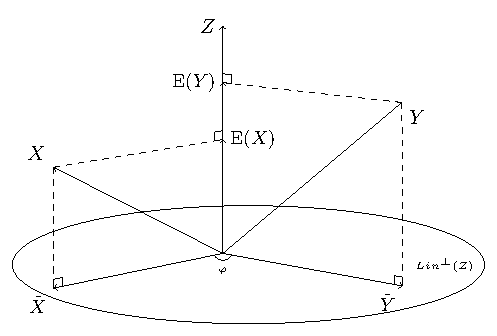
\includegraphics[width=0.55\linewidth]{figures/partial_corr.pdf}
  \caption{Partial correlation between $X$ and $Y$ while $Z$ is fixed.}
  \label{fig:pcorr_def1}
\end{figure}

\begin{definition}
Partial correlaiton between random variables $X$ and $Y$ holding random variable $Z$
fixed is the geometric mean between the coefficient $\hat \beta_{XY}$ in regression
\[
\hat X = \hat \beta_{XY} Y + \hat \beta_{XZ} Z
\]
and the coefficinent $\hat \beta_{YX}$ in regression
\[
\hat Y = \hat \beta_{YX} X + \hat \beta_{YZ} Z
\]
which has the same sign as the coefficients $\hat \beta_{XY}$ and $\hat \beta_{YX}$.
\end{definition}

Following the definition, we need to start with regressing variable $X$ onto
$Y$ and $Z$. Then, the vector we obtained $\hat X$ can be broken up into the sum of
$\hat \beta_{XY} Y$ and $\hat \beta_{XZ} Z$.
Projecting $\hat \beta_{XY} Y$ onto $Lin^{\perp}(Z)$ we results in a vector
$\alpha \widetilde Y$ where $\widetilde Y = Y - \E(Y)$ is the projection of $Y$ onto $Lin^{\perp}(Z)$.

By the properties of similar triangles
\[
\frac{\beta_{XY} Y}{Y} = \frac{\alpha \widetilde Y}{\widetilde Y} \Leftrightarrow \beta_{XY} = \alpha
\]

In the same way we perform a regression of $Y$ onto $X$ and $Z$ and repeat the
same steps as for $X$. Finally, we get the whole picture:

\begin{figure}[ht!]
\begin{center}
\subfigure[]{
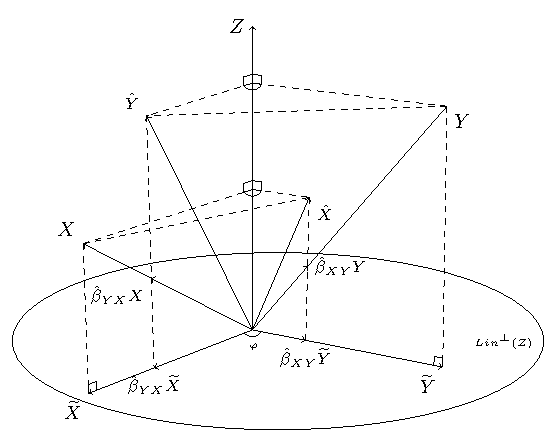
\includegraphics[width=0.55\linewidth]{figures/part_corr_2.pdf}
\label{fig:part_corr_alt}}
%\hspace{4ex}
\subfigure[]{
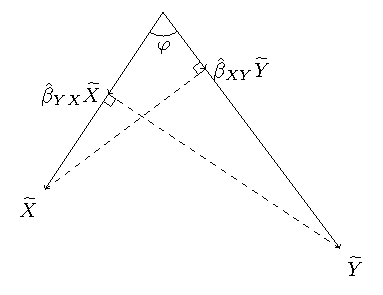
\includegraphics[width=0.35\linewidth]{figures/part_corr_2_lin.pdf}
\label{fig:part_corr_alt_lin}}
\caption{\subref{fig:part_corr_alt}: Alternative definition of the partial correlation;
\subref{fig:part_corr_alt_lin}: $Lin^{\perp}(Z)$.}
\end{center}
\end{figure}

Having plotted $Lin^{\perp}(Z)$ now we can express $\cos \varphi$ in terms of $\beta_{XY}$
and $\beta_{YX}$

\begin{equation}\label{eq:part_cor_cos}
\begin{split}
\cos \varphi &= \frac{\vert \beta_{XY} \widetilde Y \vert}{\vert \widetilde X \vert} = \vert \beta_{XY} \vert \\
\cos \varphi &= \frac{\vert \beta_{YX} \widetilde X \vert}{\vert \widetilde Y \vert} = \vert \beta_{YX} \vert \\
\cos^2 \varphi &= \vert \beta_{XY} \beta_{YX} \vert \stackrel{sign(\beta_{XY}) = sign(\beta_{YX})}{=} \beta_{XY} \beta_{YX}
\end{split}
\end{equation}

Recall that the angle $\varphi$ can be interpreted as the partial correlation
between $X$ and $Y$ holding $Z$ fixed, so it follows form equaitions~\eqref{eq:part_cor_cos}

\[
\pCorr^2(X,Y; Z) = \cos^2 \varphi = \beta_{XY} \beta_{YX}
\]

\subsection{Partial correlation as correlaiton between residuals}

\marginnote{
???
}

\begin{theorem}
Partial correlaiton between $X$ and $Y$ holding $Z$ fixed is the negative
correlaiton coefficient betwenn the residuals $\hat u$ in the regeression model
\[
X = \alpha_1 Y + \alpha_2 Z + u
\]
and the residuals $\hat v$ in the model
\[
Y = \beta_1 X + \beta_2 Z + v
\]
\end{theorem}

\begin{proof}
The first step is to find the residuals in the mentioned regresisions.
For example, in order to get $\hat u$ we regress $X$ onto $Lin(Y,Z)$
which results in $\hat X$. Then we take the difference $X - \hat X = \hat u$
and project it as well as $X$ itself onto $Lin^{\perp}(Z)$ as demonstrated
in Figure~\ref{fig:pcorr_t_x}.

Figure~\ref{fig:pcorr_t_y} shows the same step for obtainig $\hat v$.

\begin{figure}[ht!]
\begin{center}
\subfigure[]{
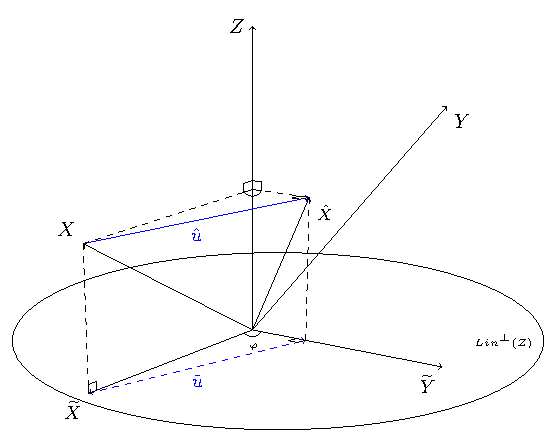
\includegraphics[width=0.45\linewidth]{figures/pcorr_theorem_x.pdf}
\label{fig:pcorr_t_x}}
%\hspace{4ex}
\subfigure[]{
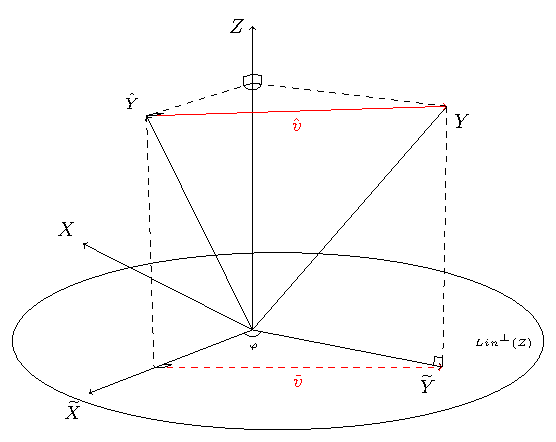
\includegraphics[width=0.45\linewidth]{figures/pcorr_theorem_y.pdf}
\label{fig:pcorr_t_y}}
\caption{\subref{fig:pcorr_t_x}: $\hat u$ form regression of x onto $Y$ and $Z$, $\hat u$ projected;
\subref{fig:pcorr_t_y}: $\hat v$ from regression of $Y$ onto $X$ and $Z$, $\hat v$ projected.}
\end{center}
\end{figure}

After all we put these figure together and the goal is to find the angle between
the red and blue lines which is the same as the angle between the dashed
red and blue lines. However, before that we need to apply translating to them to
get this angle as shown in Figure~\ref{fig:pcorr_t_lin}. Finally, using the properties of
complementary angles, angles in triangles and parallelograms
we conclude that the angle between the residuals $\tilde u$ and $\tilde v$
is eqaul to $\varphi$.

\begin{figure}[ht!]
\begin{center}
\subfigure[]{
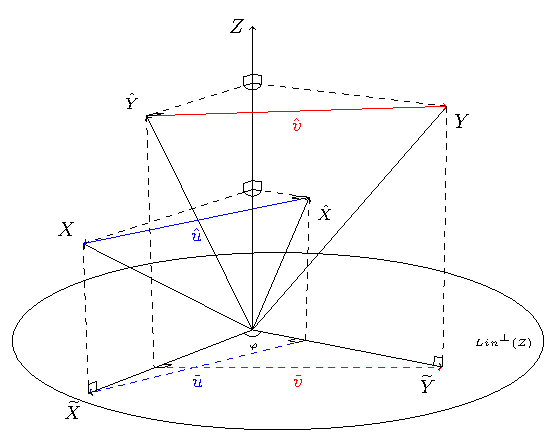
\includegraphics[width=0.45\linewidth]{figures/pcorr_t_xy.pdf}
\label{fig:pcorr_t_xy}}
%\hspace{4ex}
\subfigure[]{
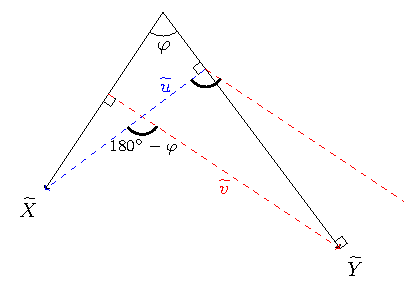
\includegraphics[width=0.45\linewidth]{figures/pcorr_t_lin.pdf}
\label{fig:pcorr_t_lin}}
\caption{\subref{fig:pcorr_t_x}: The residuals of both regressions;
\subref{fig:pcorr_t_y}: $Lin^{\perp}(Z)$.}
\end{center}
\end{figure}
\end{proof}
